\chapter{Análisis de los resultados}
En este capítulo se analiza varios aspectos de la técnica digital en contraste con la técnica tradicional buscando validar la solución propuesta y demostrar las ventajas que esta presenta.

\section{Comparación de perfiles}
Utilizando los resultados presentados en los ensayos \ref{sec:ensayo-erosion-maxima}, se comparan perfiles obtenidos con ambas técnicas con el objetivo de estudiar la bondad de la técnica digital para relevar la condición de erosión. \\
En la figura \ref{fig:comparacion-perfiles}, se muestran tres perfiles sobre el foso de erosión capturados con las tecnicas digital y tradicional. \\
En el perfil superior izquierdo, se observa que los datos continuos relevados con la cámara son aproximados de forma precisa por las mediciones con nivel óptico en condiciones donde el terreno no presenta cambios abruptos. \\
En el perfil superior derecho, se observan 3 mediciones, a 30 m, 42 m y 60 m respectivamante, que se presumen haber sido tomadas de forma incorrecta con el nivel optico. No obstante, sirve para ilustrar que la tecnica tradicional puede sufrir de errores de hasta 15 mm en prototipo, o equivalentemente, 1 m en prototipo (utilizando una escala 1:65) que no podrian ser detectados sin una superficie de referencia. Aproximadamente a los 50 m se incurre en un error de una indole distinta. En este caso, la causa de la medicion incorrecta es un cambio abrupto en la condicion del terreno, que no pudo ser detectada por el operador de la mira debido la escala del modelo. \\ 
En última instancia, se presenta el perfil inferior donde se observa el efecto de la pendiente del foso de erosión sobre una serie de mediciones con nivel. En este caso, la pendiente dificulta el apoyo del palpador sobre la superficie sin producir alteraciones, derivando en mediciones por encima del valor real. \\
Estas comparaciones ponen en evidencia que la resolución del modelo 3D obtenido con la técnica digital, es superior en zonas donde los datos relevados con la técnica tradicional no han sido cuidadosamente elegidos o el terreno es muy irregular. Cuando estos errores no están presentes, la precisión de ambas técnicas se encuentra similar.

\begin{figure}[ht]
\centering
\begin{minipage}[h]{.45\textwidth}
\begin{center}
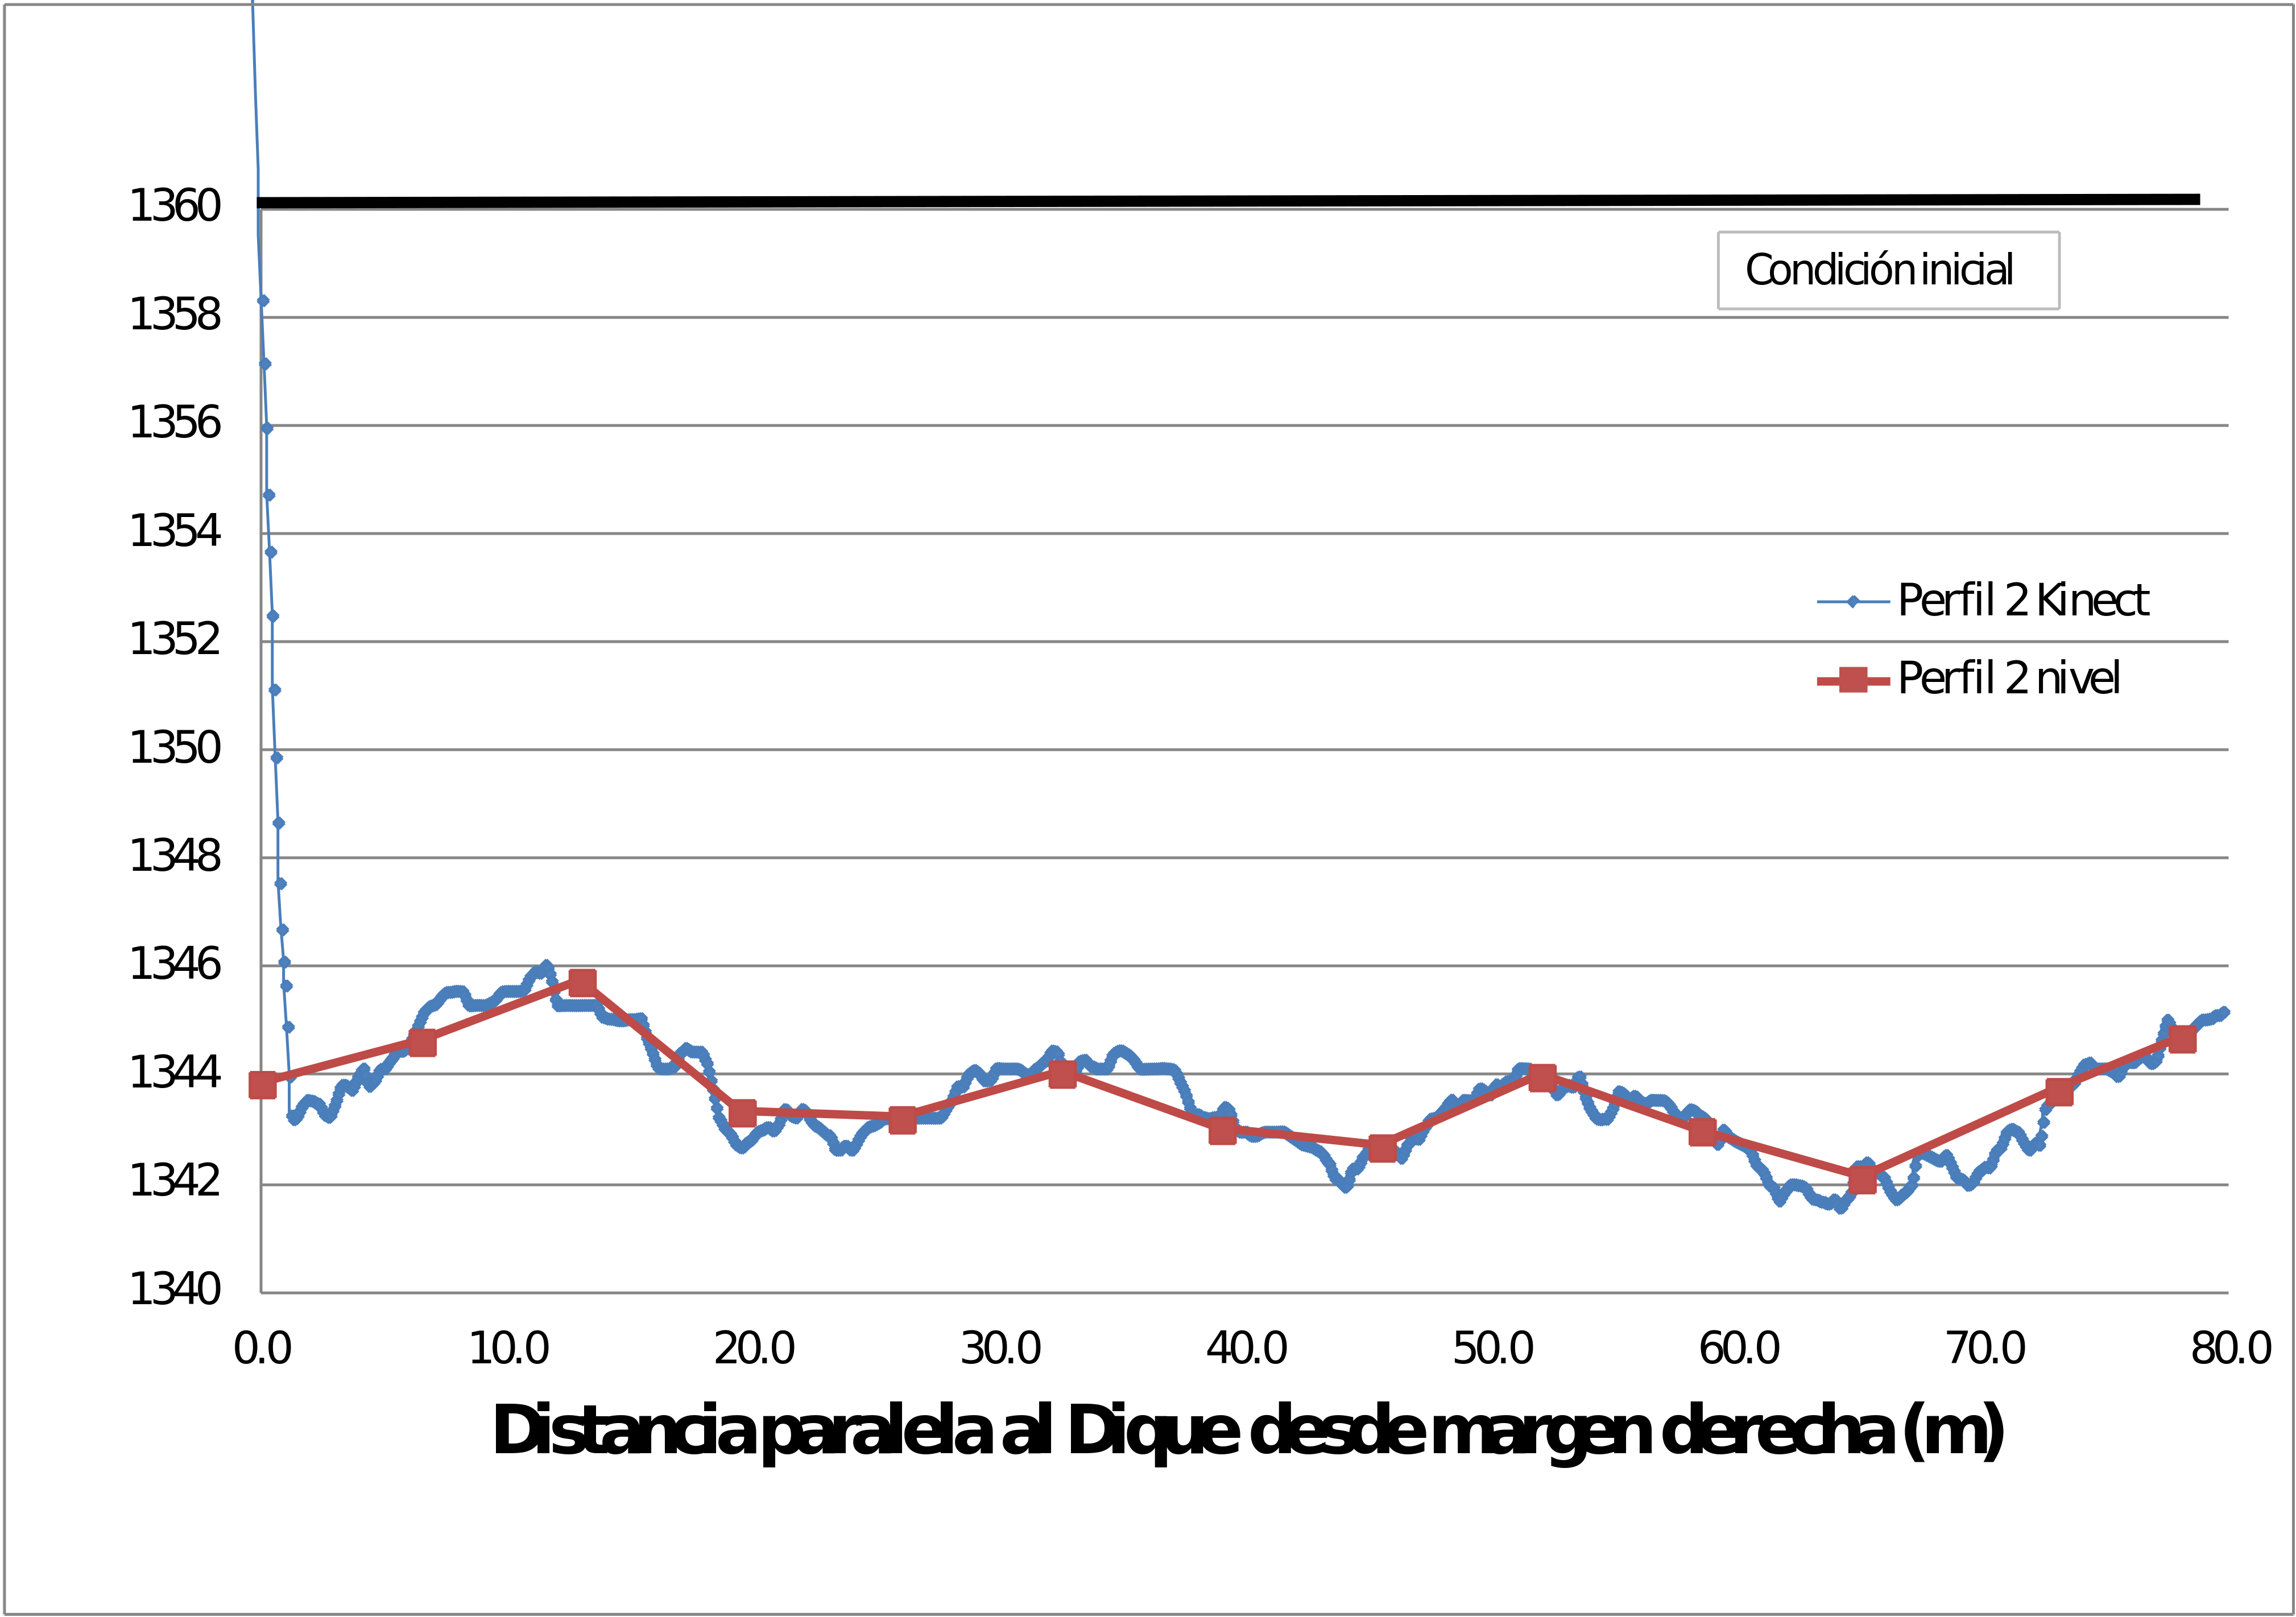
\includegraphics[width=\imsizeS]{foso-erosion-izquierda}
\end{center}
\end{minipage}
\hfill
\begin{minipage}[h]{.45\textwidth}
\begin{center}
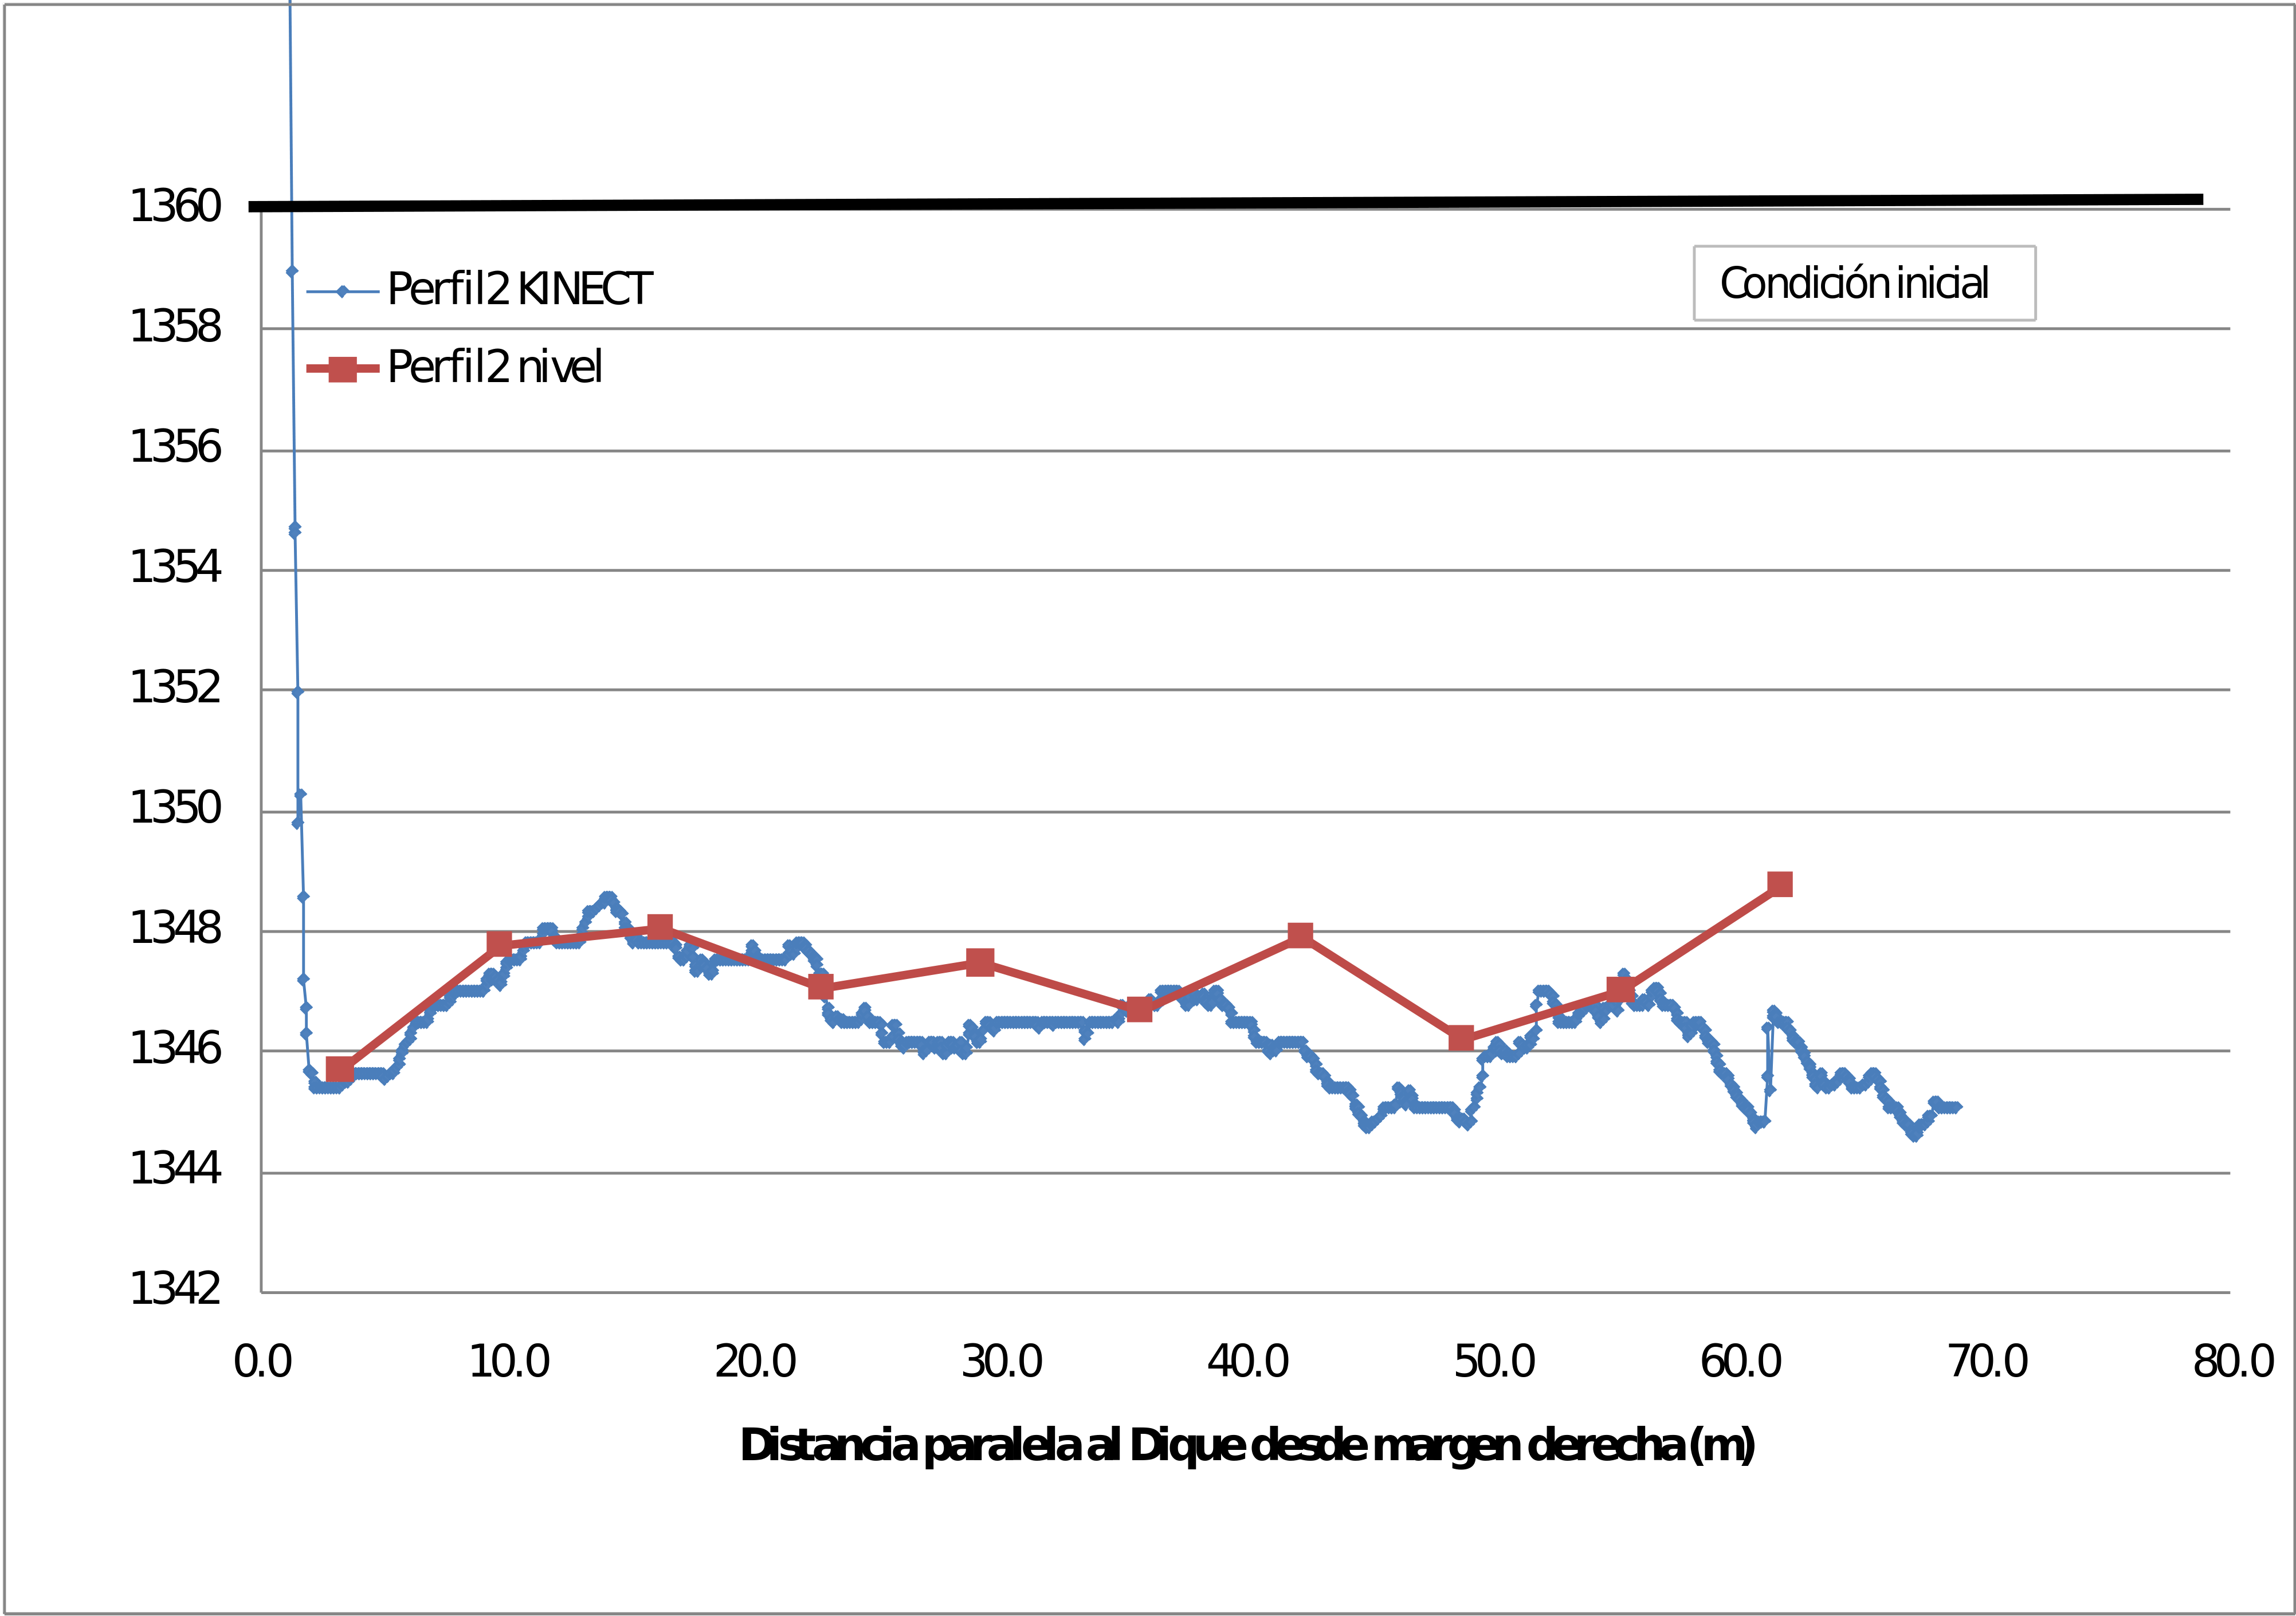
\includegraphics[width=\imsizeS]{foso-erosion-centro}
\end{center}
\end{minipage}
\hfill
\begin{minipage}[h]{.45\textwidth}
\begin{center}
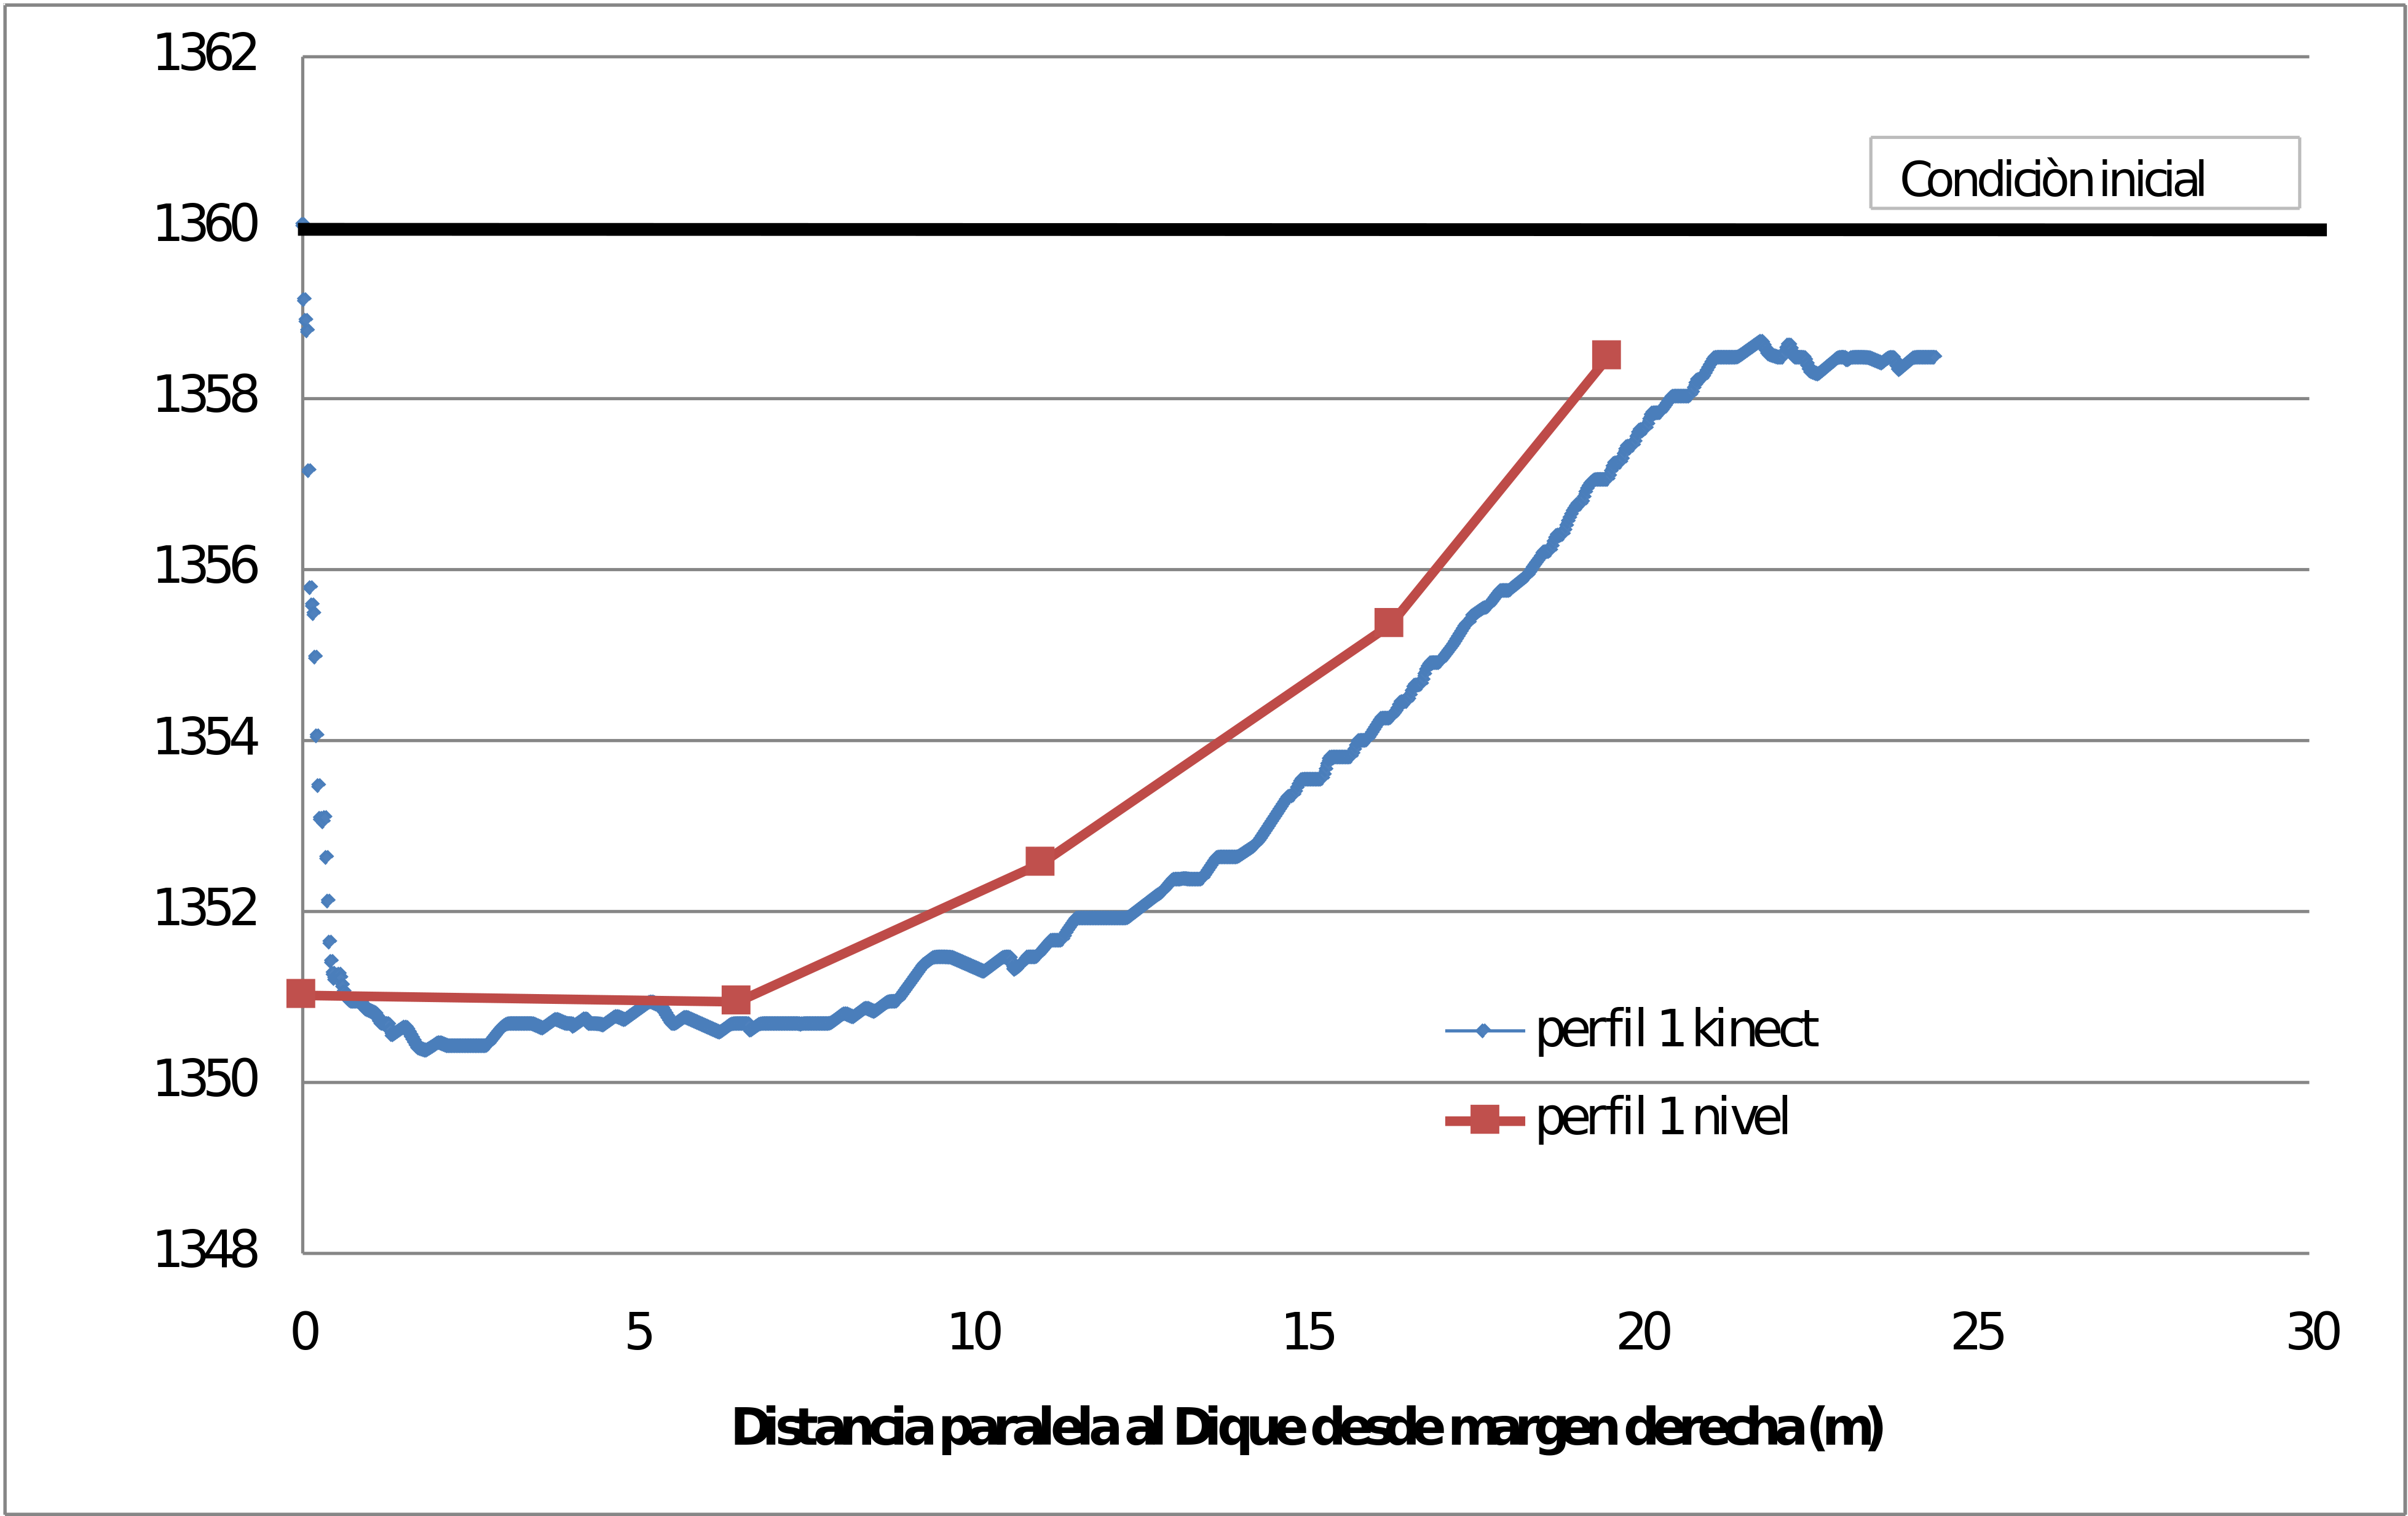
\includegraphics[width=\imsizeS]{foso-erosion-derecha}
\end{center}
\end{minipage}
\hfill
\caption[Comparación de perfiles del foso de erosión con nivel óptico y cámara Kinect]
{Comparación de perfiles del foso de erosión relevados con nivel óptico y con cámara Kinect.}
\label{fig:comparacion-perfiles}
\end{figure}

\newpage % Salto de página para acomodar las imágenes

\section{Erosión máxima}
A continuación se presentan las máximas erupciones observadas en el foso de erosión aguas abajo del canal moderador y el dique móvil relevando tanto con nivel y mira como con la cámara RGB-D.

\begin {table}[H]
\caption {Máximos niveles de erosión en el Canal Moderador} 
\label{tab:erosion-maxima-cm} 
\begin{center}

\begin{tabular}{|c|c|c|c|c|c|}
\hline 
Caudal $m^{3}/s$&Ensayo&Nivel óptico (m)&Kinect (m)&Diferencias &Diferencias\\
                &      &                &          &absolutas en &absolutas en\\
                &      &                &          &prototipo (m)&modelo (mm)\\ 
\hline 
90 & 4 & 1350.96 & 1350.37 & 0.59 & 9.07\\ 
\hline 
600 & 14 & 1349.5 & 1349.16 & 0.34 & 5.23 \\ 
\hline 
900 & 1 & 1344.8 & 1345.75 & 0.95 & 14.61\\ 
\hline 
1600 & 13 & 1345.7 & 1345.38 & \textbf{0.32} & \textbf{4.92}\\
\hline
4200 & 7 & 1345.2 & 1345.59 & 0.39 & 6\\ 
\hline 
4200 & 9 & \textbf{1344.6} & \textbf{1344.18} & 0.42 & 6.46 \\ 
\hline 
     &   &        & Promedio & 0.501 & 7.71 \\    
\hline 
     &   &        & Desv. estándar & 0.218 & 3.36 \\
\hline 
\end{tabular}
\end{center}
\end{table}

\begin {table}[H]
\caption {Máximos niveles de erosión en el Dique Móvil} 
\label{tab:erosion-maxima-dm}
\begin{center}
 
\begin{tabular}{|c|c|c|c|c|c|}
\hline 
Caudal $m^{3}/s$&Ensayo&Nivel óptico (m)&Kinect (m)&Diferencias &Diferencias\\
                &      &                &          &absolutas en &absolutas en\\
                &      &                &          &prototipo (m)&modelo (mm)\\ 
\hline 
220 & 5 & 1354.2 & 1354.89 & 0.69 & 10.61 \\ 
\hline 
600 & 14 & 1350.1 & 1349.67 & 0.43 & 6.61 \\   
\hline 
900 & 1 & 1346.1 & 1345.86 & 0.24 & 3.69 \\ 
\hline 
4200 & 7 & \textbf{1342.3} & \textbf{1343.2} & 0.9 & 13.84 \\  
\hline 
4200 & 9 & 1343.2 & 1343.41 & \textbf{0.21} & \textbf{3.23} \\
\hline 
     &   &        & Promedio & 0.493 & 7.6 \\
\hline 
     &   &        & Desv. estándar & 0.265 & 4.08 \\
\hline 
\end{tabular}
\end{center}
\end{table}

\begin{figure}[ht]
\centering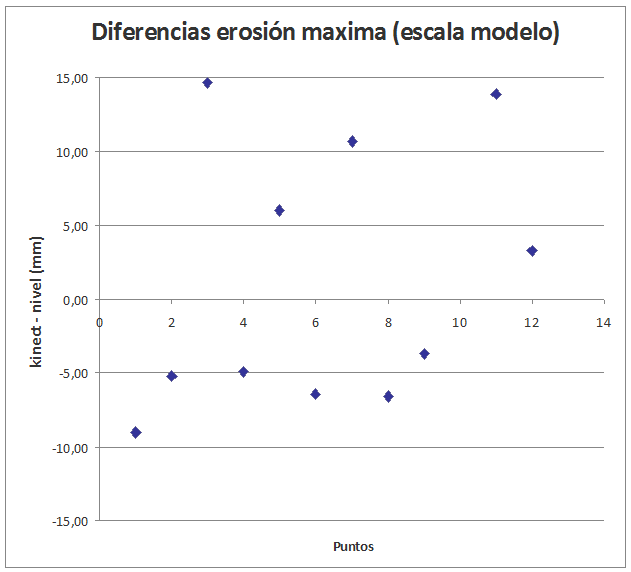
\includegraphics[width=\imsizeS]
{diferencias-erosion-maxima-modelo}
\caption[Diferencias entre mediciones de erosión máxima Kinect y Nivel]
{Diferencias (con signo) entre mediciones de erosión máxima relevadas con Kinect y con nivel óptico (en escala modelo).}
\label{fig:diferencias-erosion-maxima-modelo}
\end{figure}

Se observó un promedio en las diferencias absolutas de 7.7 mm aproximadamente y una desviación estándar de hasta 4 mm. Teniendo en cuenta que la técnica tradicional contempla errores de hasta 15 mm y el error asociado al sensor de profundidad de la Kinect es de hasta 5 mm, se considera que las mediciones realizadas con la tecnica digital estan dentro del rango aceptable para ensayos de erosión máxima. \\
Se llevó a cabo un análisis de regresión lineal simple (correlación) entre las mediciones realizadas con ambas técnicas (en escala prototipo) y se obtuvo un coeficiente de correlación $R^{2} = 0.976$, mostrando efectivamente que las mediciones entre ambas técnicas están altamente correlacionadas.

\begin{figure}[ht]
\centering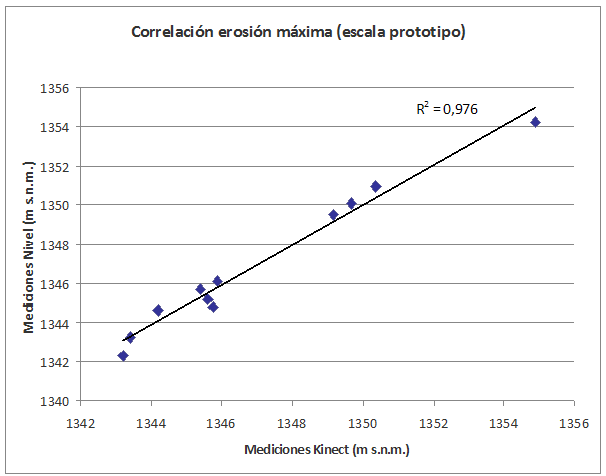
\includegraphics[width=\imsizeS]
{correlacion-erosion-maxima-prototipo}
\caption[Análisis de correlación entre mediciones de erosión máxima Kinect y Nivel]
{Análisis de correlación entre mediciones de erosión máxima Kinect y Nivel en escala prototipo. Se obtiene un $R^{2} = 0.976$.}
\label{fig:correlacion-erosion-maxima-prototipo}
\end{figure}

\section{Relevamiento de canalizaciones}

En este apartado se estudia las bondades que presenta la técnica digital para relevar el modelo físico con precisión global y se realizaron una comparación con respecto a los resultados derivados de aplicar la técnica tradicional. \\
En la sección \ref{sec:ensayo-formas-de-fondo} se presentan los resultados obtenidos para uno de los ensayos hidráulicos realizados que estudia formas de fondo generadas aguas arriba del dique para un caudal de $600 m^{3}/s$. \\
La problemática asociada a este tipo de estudios radica en la necesidad de relevar áreas extensas y con alta densidad de puntos. relevando puntos equidistantes sobre varios perfiles transversales y añadiendo la medición de puntos extras que se consideran representativos en la definición de las canalizaciones resultantes. Para obtener una aproximación global de las canalizaciones se debe generar un modelo 3D utilizando metodos de interpolacion \cite{wiki-interpolacion}.

\begin{figure}[ht]
\centering
\begin{minipage}[h]{.45\textwidth}
\begin{center}
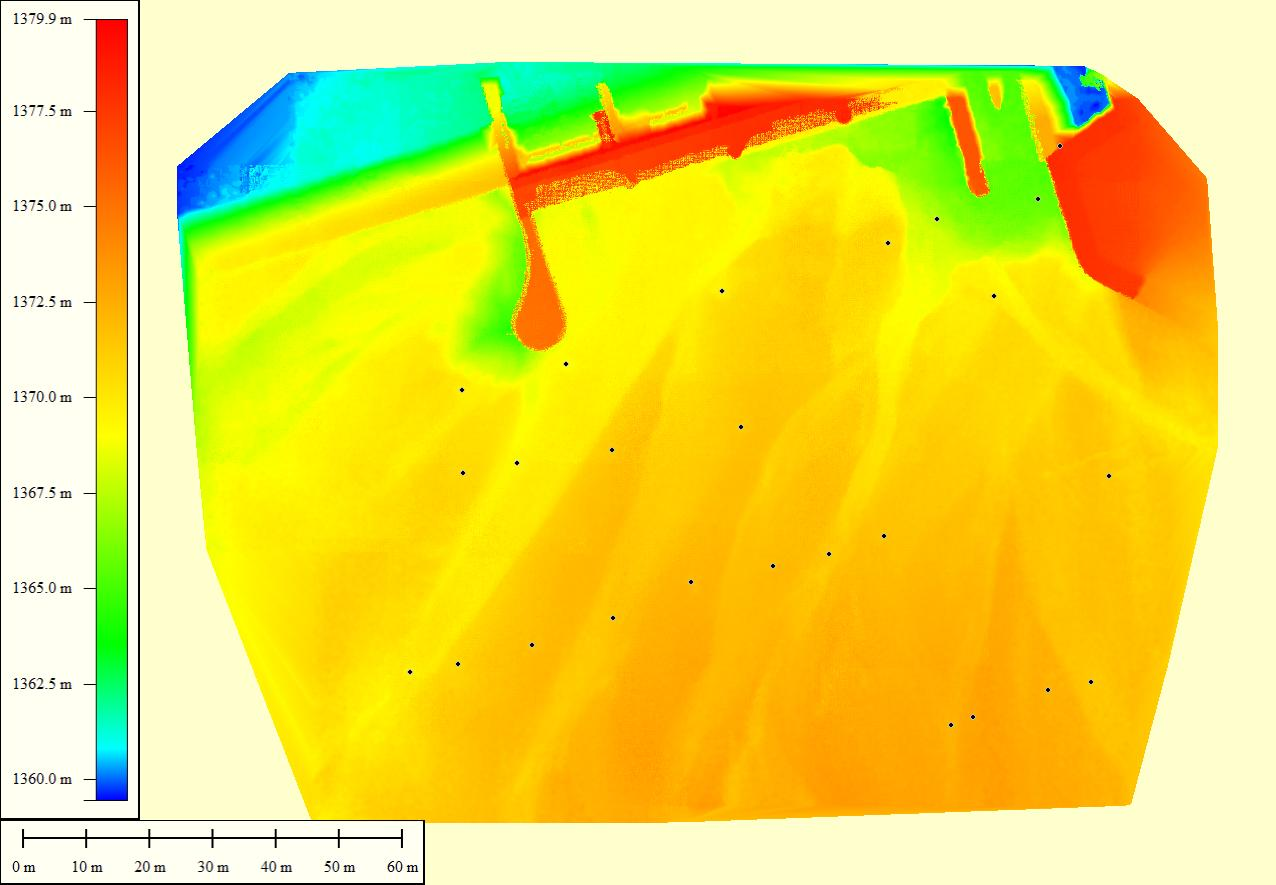
\includegraphics[width=\imsizeS]{dem-kinect}
\end{center}
\end{minipage}
\hfill
\begin{minipage}[h]{.45\textwidth}
\begin{center}
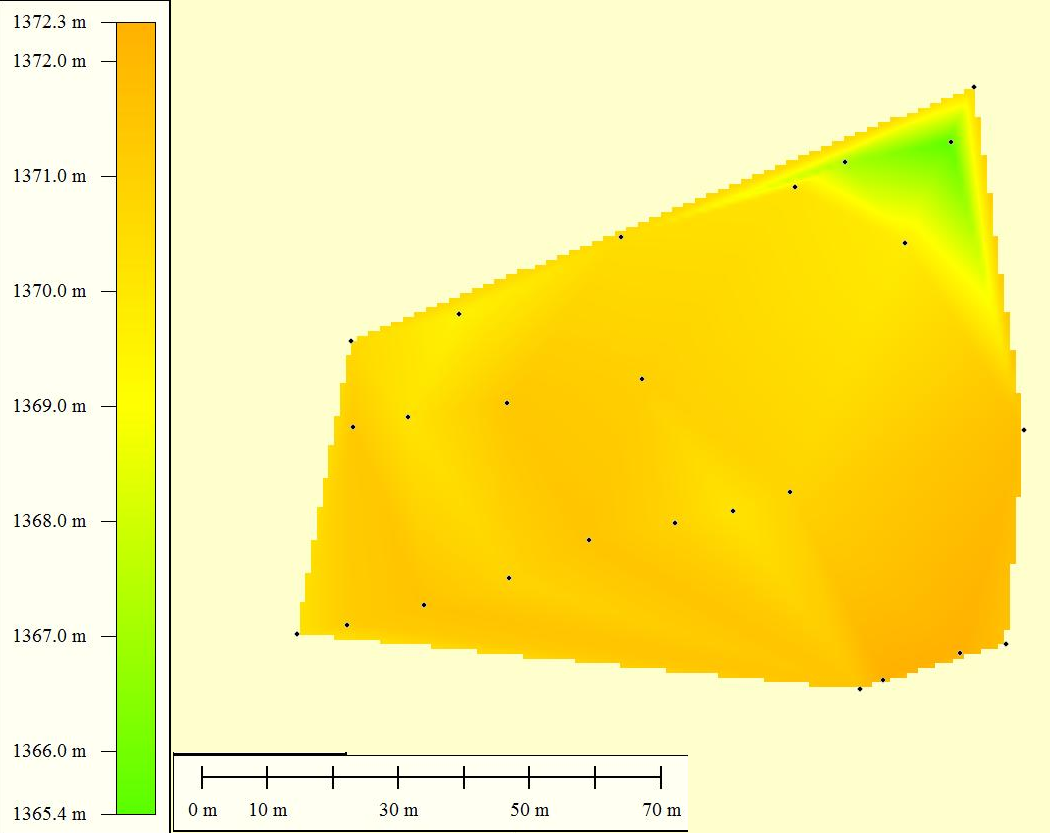
\includegraphics[width=.95\textwidth]{dem-interpolacion-nivel}
\end{center}
\end{minipage}
\hfill
\caption[DEM obtenido con Kinect y DEM generado por interpolación]
{Izquierda: DEM relevado por el sensor Kinect. Derecha: DEM generado utilizando interpolación a partir de los puntos medidos con nivel óptico. Se superponen las mediciones con nivel sobre ambos DEM's a modo ilustrativo.}
\label{fig:comparacion-dem-kinect-interpolacion}
\end{figure}

En la figura \ref{fig:comparacion-dem-kinect-interpolacion} se presentan la superficie generada por medio de interpolación a partir de puntos medidos con nivel óptico (derecha) y el modelo 3D relevado con la Kinect (izquierda) sobre la misma zona. \\
Con el objetivo de analizar la fidelidad de esta aproximacion, se trazaron un par de perfiles (sobre la misma zona), uno por cada superficie, y se calcularon las diferencias entre los resultados obtenidos con la tecnica digital y los derivados de la tecnica tradicional. En la figura \ref{fig:perfiles-diferencia-kinect-interpolacion} se presenta este experimento para cuatro cortes distintos. Se pueden apreciar zonas con diferencias de mediciones (con respecto a los valores en prototipo) dentro del intervalo $\pm0,5$ m. Este intervalo representa en modelo $\pm 7,69$ mm, lo que se considera aceptable en cuanto a la precisión de mediciones longitudinales intrusivas que se pueden alcanzar en modelos físicos. No obstante, este analisis muestra que existen dentro de estas extensas áreas relevadas, zonas donde las canalizaciones relevadas con la tecnica digital tienden a estar ubicadas entre $0,5$ m a $1,5$ m (en escala prototipo) por debajo de las canalizaciones aproximadas. Estos resultados derivan del hecho que la precision asociada a metodos de interpolacion disminuye cuando la funcion se aleja de las mediciones reales. \\
La discrepancia entre los distintos modelos 3D es demasiado alta, lo que refleja que la aproximación por interpolación no representa de forma precisa la condición real . \\
Cabe recalcar, que se puede disminuir el error presente en la superficie aproximada incrementando la cantidad de puntos relevados con la técnica tradicional (nivel y mira). Sin embargo, es simple inducir que la tecnica tradicional implica mayor tiempo de medición para relevar areas extensas con la densidad de puntos necesaria para estudios de formas de fondo. Y este proceso es tedioso cuando se deben realizar ensayos consecutivos y secuenciales asociados a aspectos complementarios del estudio global. En vista de lo anterior, se concluye que el enfoque propuesto en este trabajo permite obtener una fiel caracterizacion de las canalizaciones con un bajo costo-tiempo de medicion, resolviendo asi la problematica asociada a este tipo de ensayos. \\

\begin{figure}[ht]
\centering
\begin{minipage}[h]{.45\textwidth}
\begin{center}
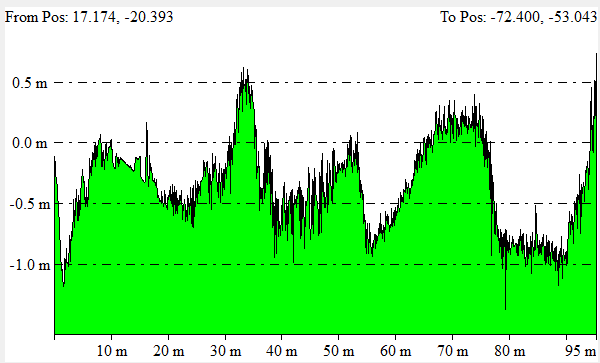
\includegraphics[width=.92\textwidth]{perfil-diferencias-kinect-interpolacion-1}
\end{center}
\end{minipage}
\hfill
\begin{minipage}[h]{.45\textwidth}
\begin{center}
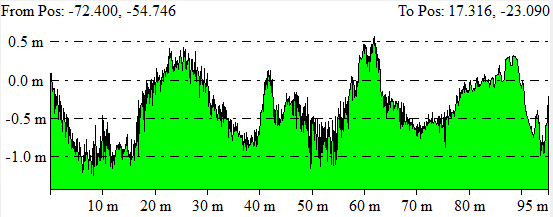
\includegraphics[width=\imsizeS]{perfil-diferencias-kinect-interpolacion-2}
\end{center}
\end{minipage}
\hfill
\begin{minipage}[h]{.45\textwidth}
\begin{center}
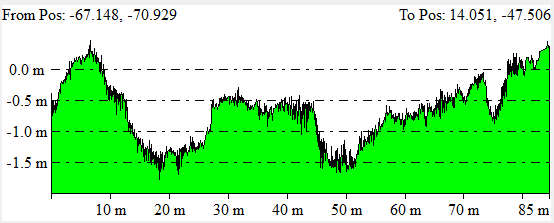
\includegraphics[width=\imsizeS]{perfil-diferencias-kinect-interpolacion-3}
\end{center}
\end{minipage}
\hfill
\begin{minipage}[h]{.45\textwidth}
\begin{center}
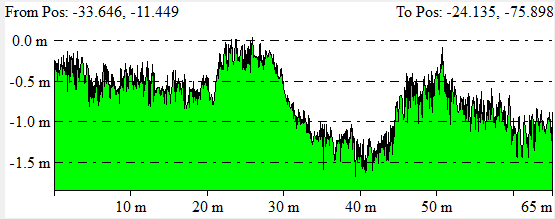
\includegraphics[width=\imsizeS]{perfil-diferencias-kinect-interpolacion-4}
\end{center}
\end{minipage}
\hfill
\caption[Diferencias entre perfiles con Kinect y perfiles extraídos desde superficie interpolada]
{Diferencias entre perfiles relevados con la técnica digital y perfiles trazados sobre una superficie interpolada a partir de mediciones con la técnica tradicional.}
\label{fig:perfiles-diferencia-kinect-interpolacion}
\end{figure}

\section{Control de estructuras del dique}

En la presente sección se analiza la precisión de la técnica propuesta para representar estructuras del dique.
En las figura \ref{fig:perfil-muro-de-encauzamiento-longitudinal}, se muestra un perfil longitudinal sobre el muro de encauzamiento. Se puede observar que la representación es precisa, conservando la forma general de la estructura, pero se advierte la presencia de algunas fluctuaciones y pequeños picos. Para analizar la magnitud del error, se trazó un perfil de menor longitud (figura \ref{fig:perfil-muro-de-encauzamiento-corto}). Se obtiene que casi todos los puntos relevados se encuentran respecto del valor 1375,1 m, el cual es la cota real de la estructura en prototipo, en el intervalo $\pm 0,3$ m (exceptuando 3 observaciones a 0,35 m, 0,4 m, 0,45 m respectivamente). Esto indica que una diferencia de 0,3 m en prototipo o equivalentemente 4.61 mm en modelo, condición que se mantiene dentro del margen esperado de 5 mm, posicionando la cámara a una distancia menor a 1,5 m (apartado \ref{sec:consideraciones-kinect}). En la figura \ref{fig:perfil-muro-de-separacion}, se traza un perfil longitudinal sobre el muro de separación del dique fijo y el canal moderador, y se obtienen valores en el intervalo 1376,27 m $\pm 0,25$ m, es decir, un error aproximado de 3,84 mm en modelo, similar a lo observado anteriormente. \\
En la figura \ref{fig:perfil-muro-de-encauzamiento-longitudinal} destacan 2 observaciones aisladas con error de aproximadamente 6 cm en escala modelo que no pudieron ser filtradas. Se propone continuar en trabajos futuros el estudio de una metodología eficaz para eliminar este tipo de \textit{outliers}. \\
Se concluye que la técnica propuesta captura con precisión aceptable las estructuras del dique, lo que habilita a poder utilizar dichas estructuras como referencias visuales en el estudio de la erosión.

\begin{figure}[ht]
\centering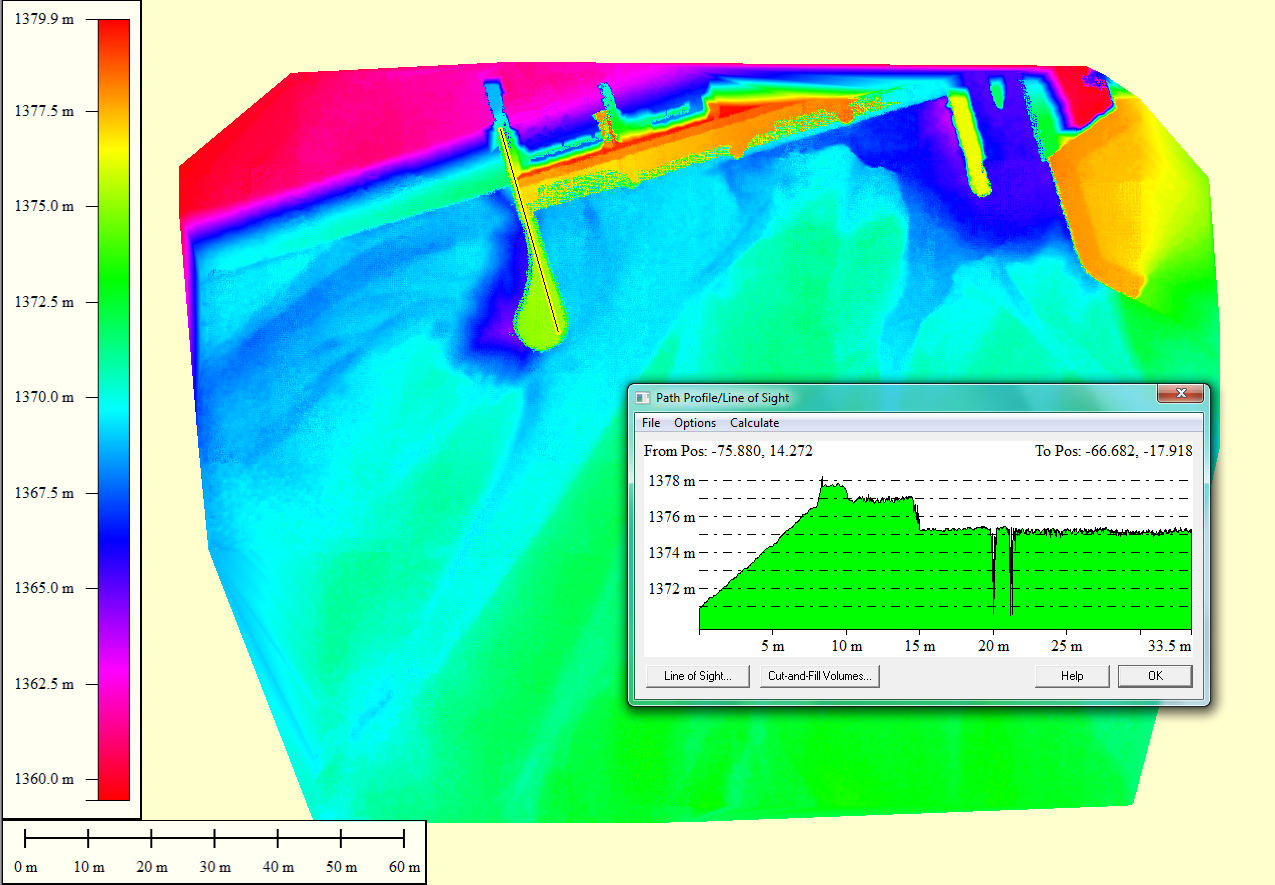
\includegraphics[width=\imsize]
{perfil-muro-de-encauzamiento-longitudinal}
\caption[Perfil longitudinal sobre el muro de encauzamiento]
{Perfil longitudinal sobre el muro de encauzamiento.}
\label{fig:perfil-muro-de-encauzamiento-longitudinal}
\end{figure}

\begin{figure}[ht]
\centering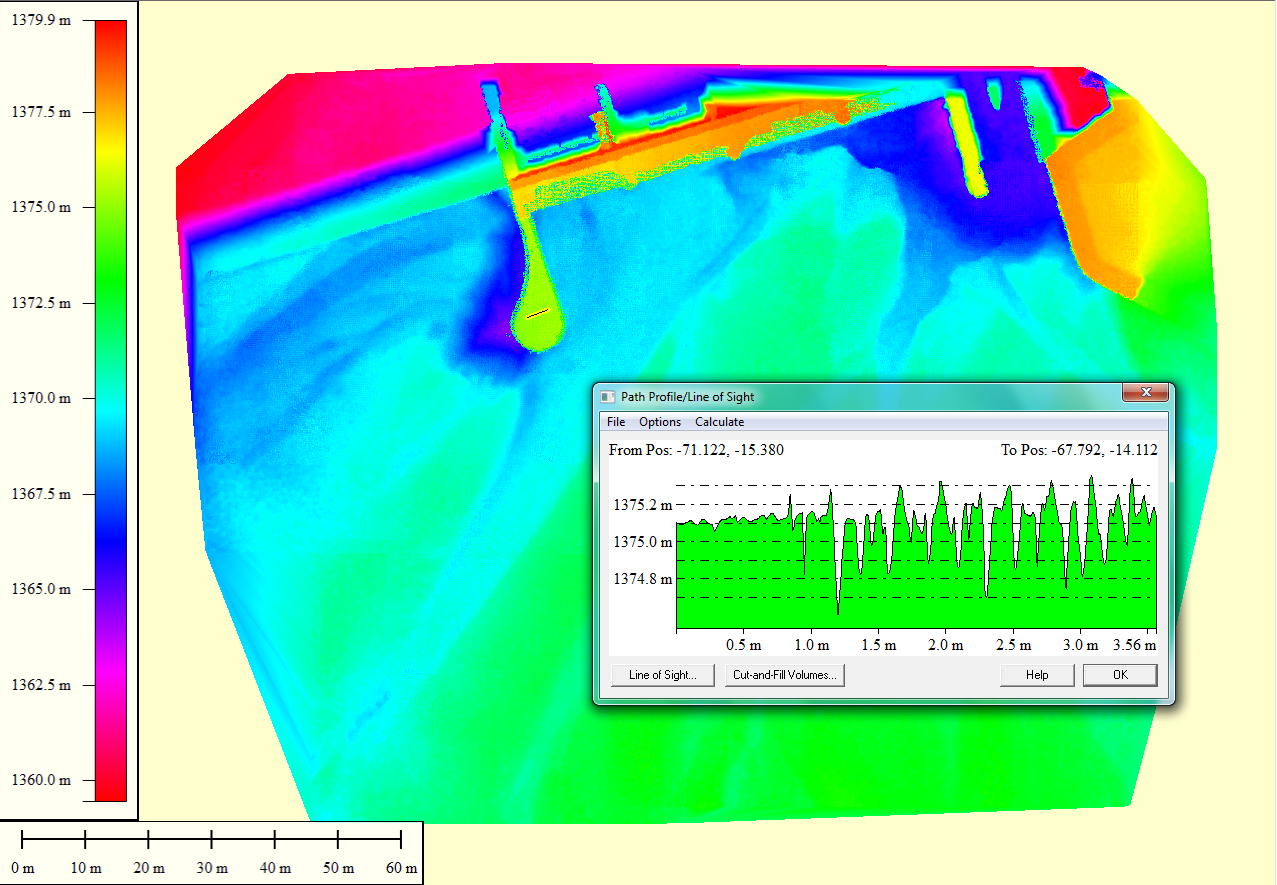
\includegraphics[width=\imsize]
{perfil-muro-de-encauzamiento-corto}
\caption[Perfil corto sobre el muro de encauzamiento]
{Perfil corto sobre el muro de encauzamiento.}
\label{fig:perfil-muro-de-encauzamiento-corto}
\end{figure}

\begin{figure}[t]
\centering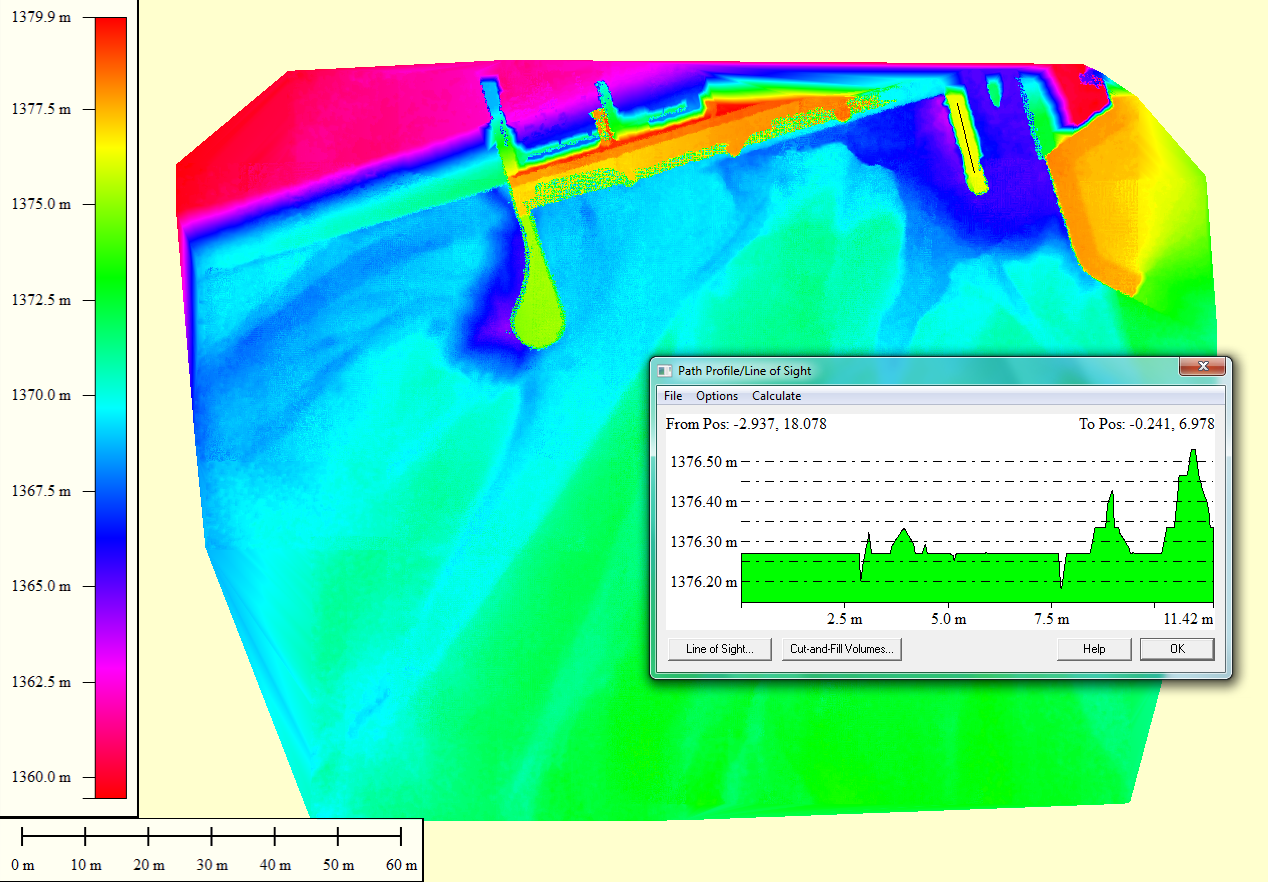
\includegraphics[width=\imsize]
{perfil-muro-de-separacion}
\caption[Perfil sobre el muro de separación entre el dique móvil y el canal moderador]
{Perfil sobre el muro de separación entre el dique móvil y el canal moderador.}
\label{fig:perfil-muro-de-separacion}
\end{figure}


